\documentclass{article}
\usepackage{framed}
\usepackage{scrextend}
\usepackage{xcolor}
\usepackage[spanish,es-tabla]{babel}
\usepackage[dvips,a3paper,centering,margin=2cm]{geometry}
\usepackage{multicol}
\usepackage{graphicx} 
\usepackage{subcaption}
\usepackage[utf8]{inputenc}
\usepackage{color}
\usepackage{float}
\usepackage{cite}
\usepackage{colortbl}
\usepackage{tabulary}
\usepackage{wrapfig}
\usepackage{multirow}
\usepackage{amsmath}
\usepackage{lipsum}
\usepackage[breaklinks=true,hidelinks]{hyperref}
\definecolor{shadecolor}{RGB}{105, 48, 195}
\definecolor{rb}{rgb}{0.025,0.5,0.9} 
\definecolor{na}{RGB}{255,255,255}
\definecolor{title}{RGB}{55, 0, 49} 
\pagestyle{empty}
\begin{document}
\vspace*{-2cm}
\changefontsizes{12pt}
\hspace*{-1cm}
\begin{minipage}{0.2\linewidth}
\vspace{0.7cm}
\vspace*{-0.15cm}
\includegraphics[scale=0.12]{images/ifir.eps}
\end{minipage}
\vspace*{-0.4cm}
\begin{minipage}{0.6\linewidth}
\vspace*{0.7cm}
\begin{center}
\changefontsizes{15pt}
\hspace*{-0.1cm}
\textbf{\textcolor{title}{Desarrollo de la plataforma “TES para tu salud” que determina los Tiempos de Exposición Solar adecuados para el tratamiento de Psoriasis en la Ciudad de México}}
\end{center}
\vspace{-0.5cm}
\begin{center}
\begin{small}
    Gamaliel López-Padilla$^1$, Adriana Ipiña$^{2}$,Rubén Piacentini$^{2}$\\
    1. Facultad de Ciencias Físico-Matemáticas,UANL, México\\
    2. Instituto de Física Rosario,CONICET-UNR, Argentina\\
    email: giovannilopez9808@gmail.com, ipina@ifir-conicet.gov.ar
\end{small}
\end{center}
\end{minipage}
\begin{minipage}{0.2\linewidth}
\hspace*{0.2cm}

\includegraphics[scale=0.2]{images/fcfm.eps}
\end{minipage}
\vspace{0.1cm}
\begin{multicols}{2}
\begin{center}
\begin{shaded}
\textbf{\textcolor{na}{Introducción}}
\end{shaded}
\end{center}
\begin{minipage}{0.4\linewidth}
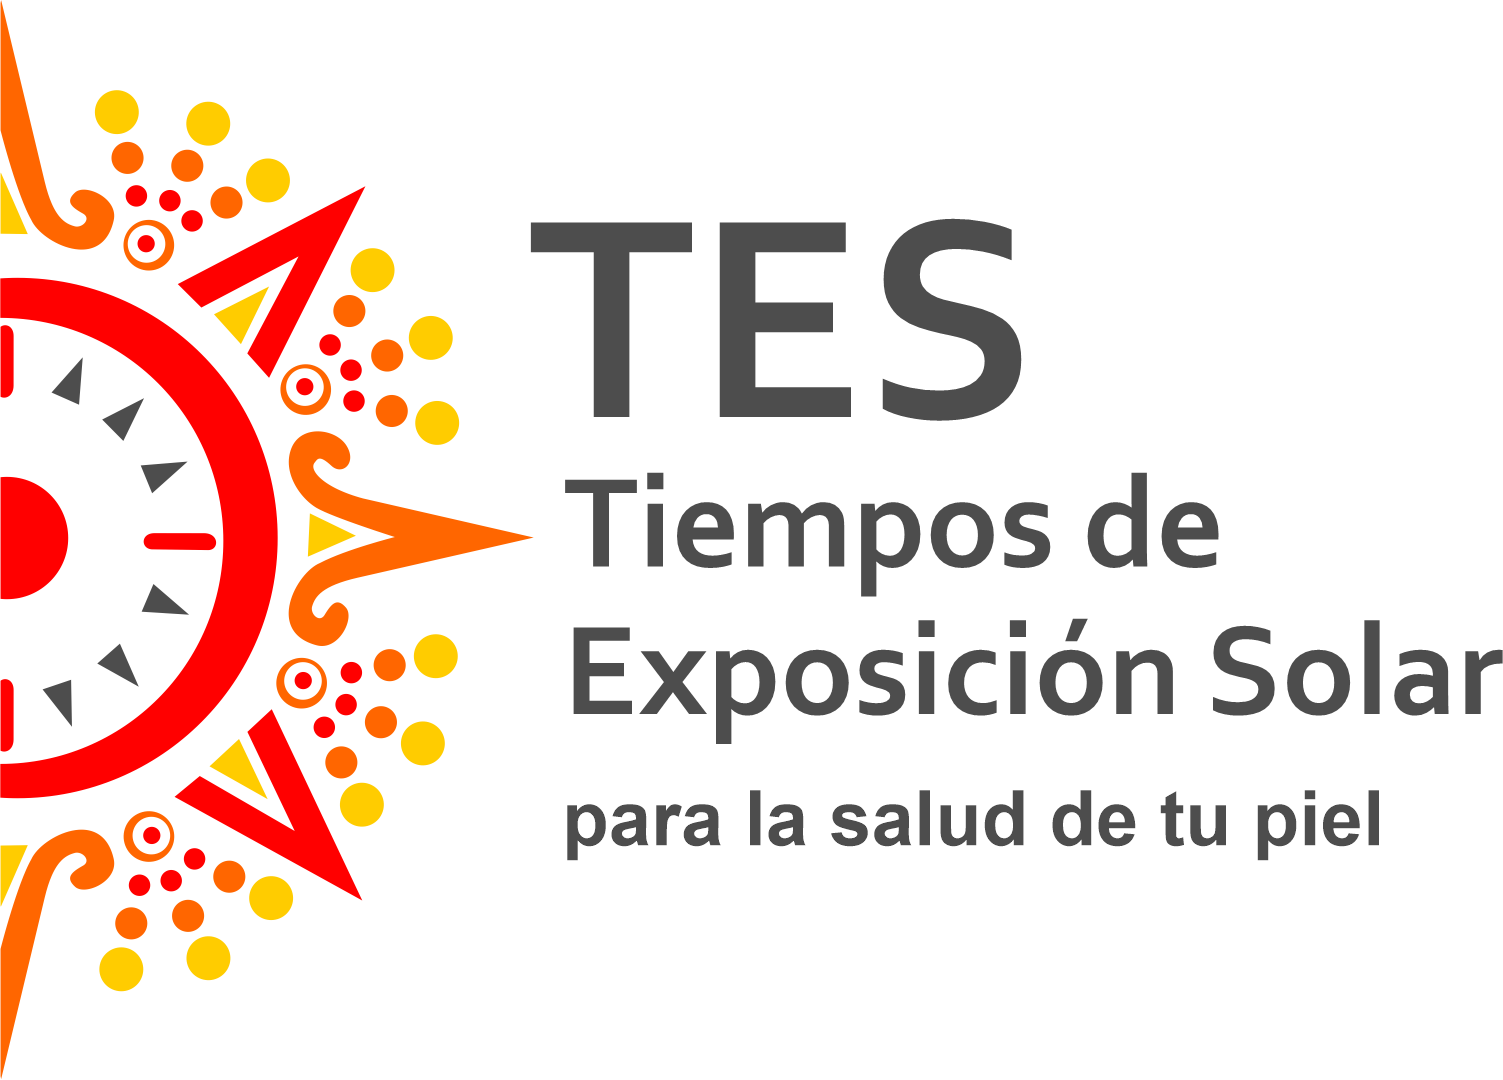
\includegraphics[scale=0.38]{images/TES.png}
\end{minipage}
\begin{minipage}{0.6\linewidth}
La Psoriasis es una enfermedad dermatológica crónica de apariencia de piel engrosada, que suele ser 
tratada con fototerapia ultravioleta (UV). Los pacientes son expuestos a fuentes artificiales UVA (320-400nm) 
siendo ésta la modalidad más utilizada en los Centros médicos. Sin embargo,
\end{minipage} \vspace{-0.1cm}\\por diversos motivos los pacientes no tienen acceso a estos tratamientos o no pueden asistir con 
la asiduidad para recibirlo adecuadamente. Una recomendación alternativa es exponerse al sol. En este trabajo presentamos 
una plataforma que calcula los tiempos de exposición solar (TES) para el tratamiento de psoriasis y TES límite para evitar quemadura, usando mediciones de irradiancia solar 
UVA y eritémica para días de cielo despejado en la Ciudad de México en el periodo 2016-2018.
\begin{center}
\begin{shaded}
\textbf{\textcolor{na}{Metodología}}
\end{shaded}
\end{center}
Para el cálculo de los tiempos de exposición solar se tomaron como referencia las mediciones de irradiancia UVA y eritémica
 para cada fototipo cutáneo, que se muestra en la tabla \ref{tabla:fototipo}.
\vspace{-0.5cm}
    \begin{table}[H]
    \centering \normalsize
    \begin{tabulary}{1.0\linewidth}{ccccccc}
         \multirow{2}{*}{Fototipo}& \multirow{2}{*}{MED (J/m\textsuperscript{2})} & \multicolumn{4}{c}{Color} & Distribución en el color de piel\\
         & & \multicolumn{4}{c}{de piel} &en la población mexicana(\%) \\  \hline
        I 	&200	&\cellcolor[RGB]{251, 244, 227}\hspace*{0.05cm} 	&\cellcolor[RGB]{245, 240, 218}\hspace*{0.05cm}  &\cellcolor[RGB]{247, 238, 217}\hspace*{0.05cm} 	&\cellcolor[RGB]{248, 234, 209} \hspace*{0.05cm} &0.8	\\ \hline
        II 	&250	&\cellcolor[RGB]{248, 234, 208}	&\cellcolor[RGB]{247, 231, 206} &\cellcolor[RGB]{247, 223, 199}	&\cellcolor[RGB]{245, 222, 188}	& 3.9 \\ \hline
        III &300 	&\cellcolor[RGB]{245, 221, 188}	&\cellcolor[RGB]{238, 213, 170} &\cellcolor[RGB]{219,182,137}	&\cellcolor[RGB]{220,170,120} &24.0	\\ \hline
        IV 	&450	&\cellcolor[RGB]{219, 191, 129}	&\cellcolor[RGB]{208, 171, 107} &\cellcolor[RGB]{193, 150, 90}	&\cellcolor[RGB]{182, 135, 75}&59.2	\\ \hline
        V	&600	&\cellcolor[RGB]{172, 121, 68}	&\cellcolor[RGB]{135, 92, 50}  &\cellcolor[RGB]{113, 70, 38}	&\cellcolor[RGB]{77, 48, 28}&8.9	\\ \hline
        VI 	&1000 	&\cellcolor[RGB]{68, 37, 20}	&\cellcolor[RGB]{43, 25, 8}  &\cellcolor[RGB]{32, 12, 7}	&\cellcolor[RGB]{10, 2, 5}	&2.5	\\ \hline
    \end{tabulary}
    \caption{{Adaptación de la clasificación de Fitzpatrick para: fototipos, 
    dosis eritémica mínima en J/m\textsuperscript{2} (MED), color de piel y sus 
    respectivos porcentajes que se presentan en la población mexicana.{\label{tabla:fototipo}}}}
    \end{table}
 Los datos de irradiancia solar fueron obtenidos a partir de mediciones minuto a minuto en el periodo de 2016-2018 de 
 10 estaciones del Sistema de Monitoreo Atmosférico (SIMAT) de la Ciudad de México. Se realizó un filtrado de estos datos para
 obtener unicamente los días de cielo despejado. A partir de los días seleccionados se creó una base de datos anual para determinar
  la irradiancia solar en tres condiciones de cielo, utilizando el factor C\textsubscript{f}: 1, 0.7, 0.5; para día despejado, medio nublado y nublado, respectivamente
   (Figura \ref{fig:cloud})
 \begin{figure}[H]
    \centering
    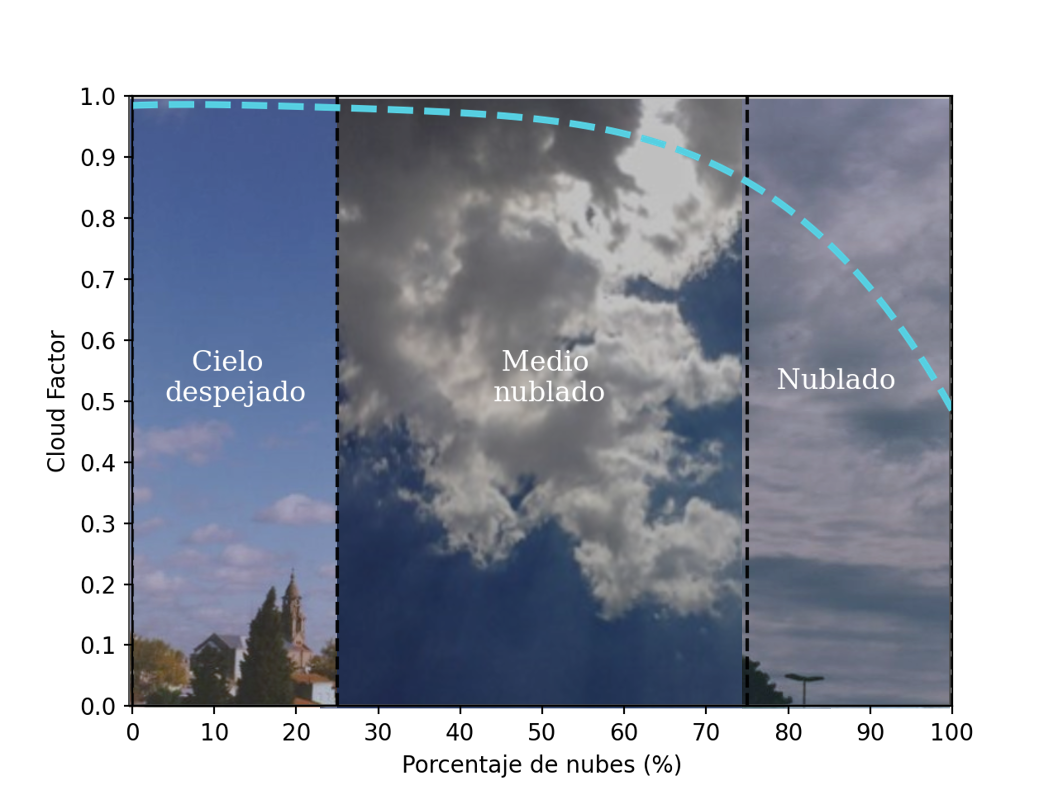
\includegraphics[scale=0.68]{images/nubes.png}
    \caption{Factor de nubes (C\textsubscript{f}) que atenúa la irradiancia solar UV, en
    función del porcentaje de cobertura en el cielo. }
    \label{fig:cloud}
\end{figure}
En cabina de fototerapia, las dosis UVA aplicadas para el tratamiento de Psoriasis son 1, 1.5, 2 y 3 J/cm$^2$. 
Para obtener la misma dosis a partir de la irradiancia solar se utilizó la siguiente ecuación:
\begin{equation*}
    Dosis_{UVA}=\int\limits_{t_0}^t\int\limits_{320nm}^{400nm} C_f E_{\lambda} d\lambda dt =\int\limits_{t_0}^{t} C_f I_{UVA}dt
\end{equation*}
donde $t_0$ y $t$ son la hora de inicio y hora de finalización para obtener la dosis UVA deseada, 
por lo tanto, $t-t_0$ es el TES requerido para el tratamiento.\\ Para evitar quemadura solar o eritema se determina el TES máximo 
empleando los MED reportados en la tabla \ref{tabla:fototipo} realizando la operación semejante a la dosis UVA incluyendo la ecuación del espectro de sensibilidad eritémica E\textsubscript{erit} de la piel humana
\begin{equation*}
    Dosis_{Erit}=\int\limits_{t_0}^{t} \int\limits_{280nm}^{400nm} \left( C_f E_{erit}E_{sol}\right)d\lambda dt = \int\limits_{t_0}^{t}C_f I_{erit}dt
\end{equation*}
\vspace{0.05cm}
\begin{center}
    \begin{shaded}
    \textbf{\textcolor{na}{Resultados}}
    \end{shaded}
    \end{center}
\begin{figure}[H]
    \begin{subfigure}[H]{0.5\linewidth}
        \centering
        \vspace{-0.1cm}
        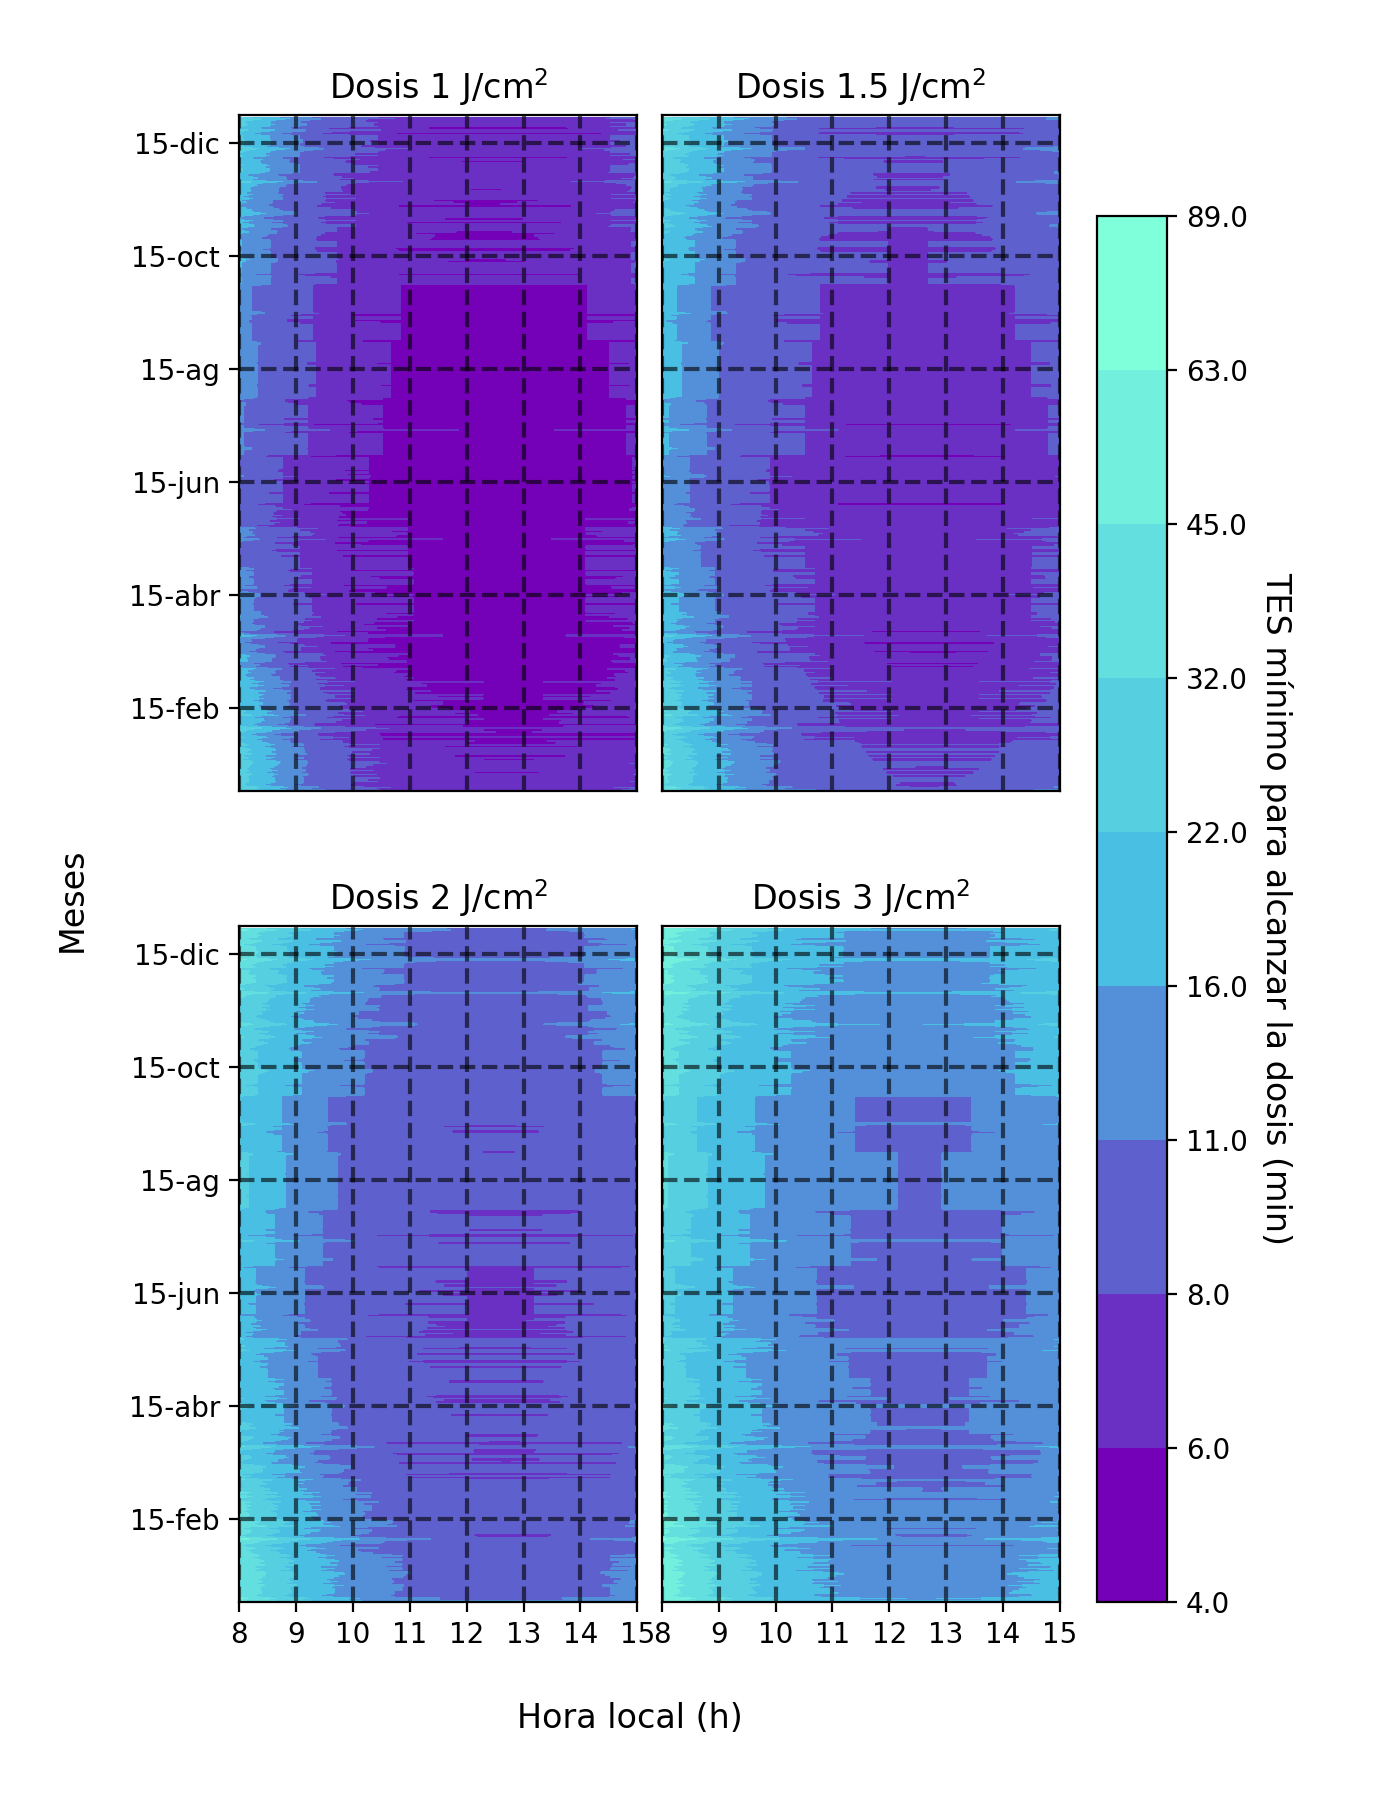
\includegraphics[scale=0.38]{images/pso.png}
    \end{subfigure}
    \begin{subfigure}[H]{0.4\linewidth}
        \centering
        \vspace{-0.2cm}
        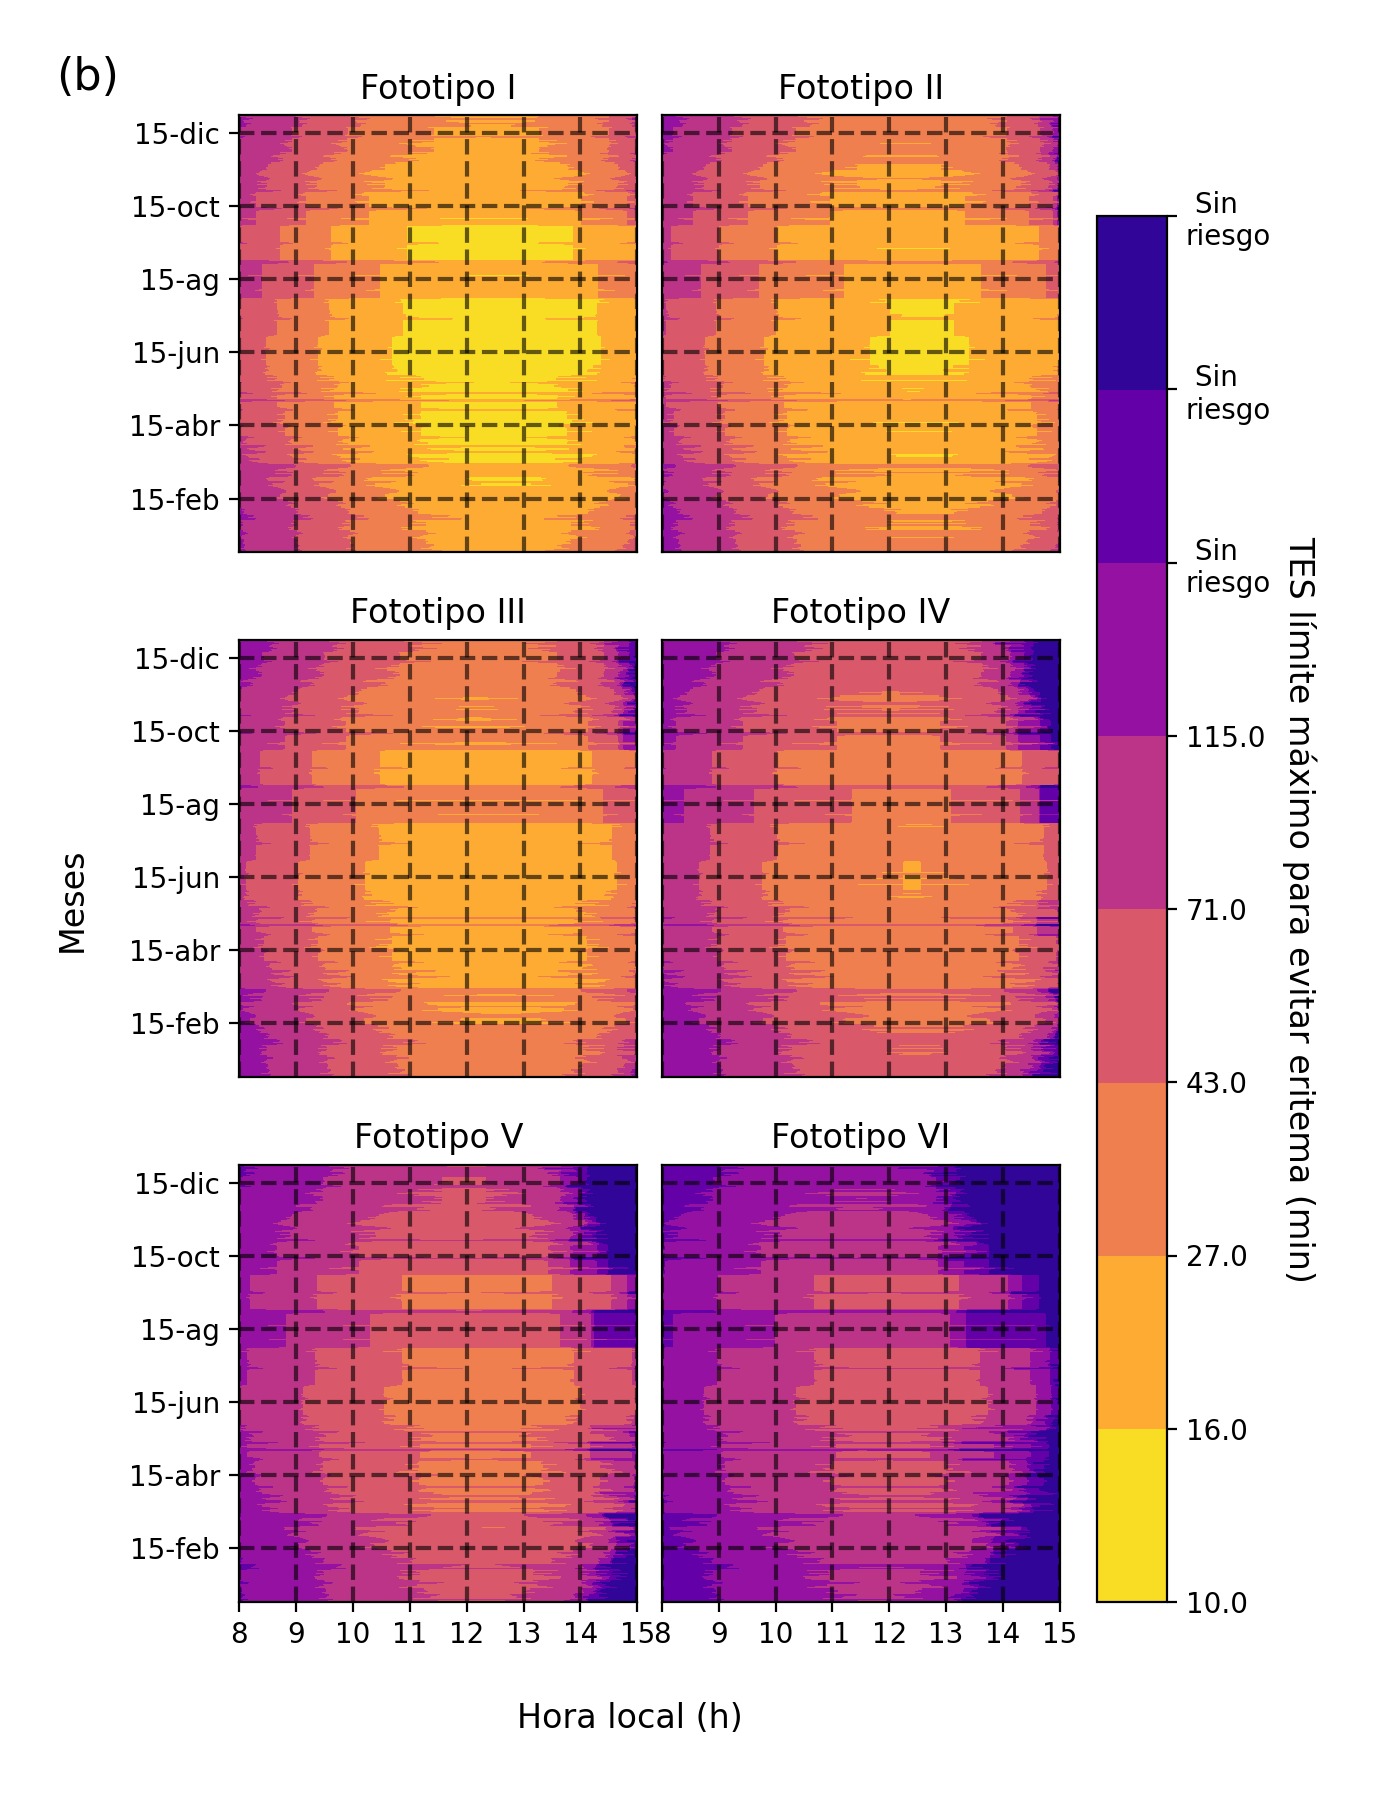
\includegraphics[scale=0.38]{images/ery.png}
    \end{subfigure}
\caption{(a) TES para obtener las dosis UVA necesarias en el tratamiento de Psoriasis y 
(b) TES para evitar eritema en cada fototipo de piel según las condiciones de cielo despejado.}
\end{figure}
\begin{center}
\begin{shaded}
\textbf{\textcolor{na}{Conclusiones}}
\end{shaded}
\end{center}
\begin{itemize}
    \item Independientemente de las condiciones de cielo, las dosis UVA para el tratamiento de Psoriasis pueden ser alcanzados en tiempos cortos durante todo el año.
    \item La diferencia entre el TES requerido para las dosis UVA y el TES para producir eritema es suficientemente grande para garantizar el tratamiento evitando el riesgo de quemadura.
    \item Esta plataforma y la asistencia remota pueden coadyuvar a realizar los tratamientos 
    dermatológicos a distancia, respondiendo a la nueva normalidad ocasionada por el virus SARS-CoV2.
\end{itemize}
\begin{center}
\begin{shaded}
\textbf{\textcolor{na}{Referencias}}
\end{shaded}
\changefontsizes{7pt}
% \bibliographystyle{abbrv}
% \nocite{*}
% \bibliography{main}
\begin{enumerate}
\item Cie standard s 013/e:2003 international standard global solar uv index. Color Research \& Application, 29(2):164–164, 2004.
\item  S. Cabrera, A. Ipiña, A. Damiani, R. R. Cordero, and R. D. Piacentini. Uv index values and trends
in santiago, chile (33.5 ° s) based on ground and satellite data. Journal of Photochemistry and
Photobiology B: Biology, 115:73 – 84, 2012.
\item  W. Kirch, editor. Global Solar UV Index, pages 500–500. Springer Netherlands, Dordrecht, 2008.
\item M. Makgabutlane and C. Y. Wright. Real-time measurement of outdoor worker’s exposure to solar
ultraviolet radiation in pretoria, south africa. South African Journal of Science, 111(5/6):1–7, May
2015.
\item H. Staiger and P. Koepke. Uv index forecasting on a global scale. Meteorologische Zeitschrift,14(2):259–270, 05 2005.
\end{enumerate}
\end{center}
\end{multicols}
\end{document}